\documentclass[10pt]{article}

\usepackage[T1]{fontenc}
\usepackage[utf8]{inputenc}
\usepackage{lmodern}
\usepackage[margin=0.85in,top=0.75in,bottom=0.8in]{geometry}
\usepackage{graphicx}
\usepackage{booktabs}
\usepackage{caption}
\usepackage{amsmath}
\usepackage{textcomp}
\usepackage{microtype}
\usepackage{xcolor}
\usepackage[colorlinks=true,linkcolor=black,citecolor=black,urlcolor={blue!50!black}]{hyperref}
\usepackage{enumitem}
\usepackage{fancyhdr}
\usepackage{titlesec}

\raggedbottom
\setlength{\parindent}{0pt}
\setlength{\parskip}{4.5pt}
\captionsetup{font=footnotesize,labelfont=bf,skip=3pt}
\titlespacing*{\section}{0pt}{9pt}{3pt}
\titlespacing*{\subsection}{0pt}{7pt}{2pt}

\pagestyle{fancy}
\fancyhf{}
\renewcommand{\headrulewidth}{0pt}
\fancyfoot[C]{\small\thepage}

\title{\vspace{-1.5em}\textbf{Benchmarking Protein--Protein Interface Prediction on Experimental versus AlphaFold-Predicted Structures}}
\author{Armeen Shasti-Nazem}
\date{}

\begin{document}
\maketitle
\thispagestyle{fancy}
\vspace{-2.2em}

\section*{Abstract}

PeSTo is a geometric deep-learning model that predicts protein--protein
interface residues from atomic coordinates, trained only on experimentally
determined structures. Because most protein structures available today are
AlphaFold predictions, we ask whether PeSTo's accuracy transfers to AlphaFold
input. Starting from PDB complexes released after AlphaFold2's training
cutoff and filtered to under 30\% sequence identity to
PeSTo's own training, validation, and test sequences, we assembled a primary
benchmark set of 566 protein chains with both an experimental and
an AlphaFold structure, a validated residue mapping, and interface labels,
and ran PeSTo on each chain's isolated experimental structure and on the
matched AlphaFold model trimmed to the same residue range. Across
554 chains with defined metrics, PeSTo's
per-chain area under the precision--recall curve (AUPR) was higher on
experimental input by a median of 0.027 (95\% CI
[0.019, 0.035], Wilcoxon $p=$$3.5\times10^{-17}$), consistent in direction across
eight strata and under an alternative buried-surface-area interface
definition. The gap was far from uniform: within AlphaFold's own confidence
bands, the pooled AUPR gap shrank from 0.254 in the lowest-confidence
residues to 0.039 in the highest-confidence residues, and a per-residue
regression associated both AlphaFold confidence (pLDDT) and local structural
divergence with each residue's prediction shift, independently of
one another and of solvent exposure. Chain length was not associated with the
size of the drop. These results describe a modest but consistent,
confidence-linked accuracy cost when applying PeSTo to AlphaFold structures,
concentrated in the flexible, lower-confidence regions where many interfaces
occur; all reported relationships are associations, not demonstrated causes.

\section{Introduction}

Protein--protein interactions underlie nearly all cellular processes, from
signal transduction to immune recognition, and the specific residues that form
a binding interface are relevant to understanding disease mutations and to
structure-based drug design \cite{zhang2024}. Determining an interface
experimentally, by solving the structure of a complex, remains slow relative to
the scale of the problem: the Protein Data Bank (PDB) holds on the order of
$2\times10^5$ structures, while the AlphaFold Protein Structure Database now
provides predicted structures for over $2\times10^8$ sequences
\cite{jumper2021,varadi2024}. Several geometric deep-learning methods now
predict interface residues directly from a single protein's three-dimensional
coordinates, without requiring a solved complex: PeSTo represents atoms by
element and position alone \cite{krapp2023}, and ScanNet extracts learned
geometric and biochemical descriptors \cite{tubiana2022}. These models are
trained on experimentally determined structures, and applying them to
AlphaFold predictions implicitly assumes the predicted geometry is close
enough to the true structure that the model's learned decision boundary still
applies.

That assumption is worth checking directly. AlphaFold reports a per-residue
confidence score, pLDDT, and its documentation states that residues scoring
below 70 may have unreliable backbone placement; low-confidence regions are
disproportionately surface-exposed loops and chain termini, which is where
many binding interfaces occur. Independent structural comparisons find that
even confidently predicted regions can deviate from experimental structures by
several tenths of an \r{A}ngstrom at longer range \cite{terwilliger2024}. Yuan
et al.\ benchmarked PeSTo and ScanNet on structures predicted by ESMFold, a
protein-language-model-based structure predictor distinct from AlphaFold, and
reported PeSTo's AUPR falling from 0.797 on experimental structures to 0.691 on
ESMFold structures \cite{yuan2024,lin2023} -- a substantial drop, but not a
direct measurement of AlphaFold specifically, whose error characteristics
differ from ESMFold's.

This paper reports a matched, AlphaFold-specific benchmark of PeSTo together
with an error analysis of where and why any accuracy gap occurs. We ask two
questions: (1) how much does PeSTo's interface-prediction accuracy change when
the input is an AlphaFold model of a chain rather than that chain's own
experimental structure, holding the chain and the ground-truth interface
fixed; and (2) is that change associated with AlphaFold's own confidence score
and with the local geometric divergence between the two structures. Both
analyses were pre-registered: endpoints, statistical tests, and descriptive
strata were fixed in writing before either comparison was computed against
real predictions, so that the reported result was not tuned after the fact.
This extends prior experimental-to-predicted transferability work (including
Yuan et al.'s ESMFold benchmark, and PeSTo's own authors' preliminary
AlphaFold exploration) to a controlled, AlphaFold-specific comparison with a
paired error analysis; it is not the first study to raise this general
concern.

\section{Methods}

\subsection{Dataset construction}

Candidate protein chains were drawn from PDB entries released after
2018-04-30, AlphaFold2's own training-data cutoff, so that the
experimental structures used here could not have been memorized during
AlphaFold's training. Candidates were restricted to crystal structures at or
better than 2.5\,\r{A} resolution, complexes of at most
10 distinct protein entities (excluding assemblies too
large for a single well-defined pairwise interface, e.g.\ viral capsids), and
chains whose polymer entity sequence is at least 40 residues
long (the entity's full expressed/construct sequence, not the count of
residues actually resolved in the deposited coordinates, which is often
substantially smaller). This search returned
8,808 PDB entries and 22,887 candidate protein chains
(Fig.~\ref{fig:attrition}). Redundant chains were then collapsed by MMseqs2
sequence clustering to 3,009 non-redundant representatives, one per
cluster.

Because PeSTo was trained on essentially all biological assemblies in the PDB,
filtering by exact PDB identifier is not sufficient: a chain released after
2018 can still be a close sequence homolog of something PeSTo has already seen
under a different identifier. Each representative was therefore searched by
MMseqs2 against the union of PeSTo's published training, validation, and test
sequence sets; 77\% of representatives matched at or above
30\% sequence identity to that union and were treated as
leakage. The leakage-free candidate set carried forward into the rest of the
pipeline is the 696 representatives below this threshold; not
all of them survive the remaining processing steps below, which is why this
paper distinguishes the leakage-free candidate set (696) from
the smaller primary benchmark set that is actually analyzed in Section~3
(566, defined below).

For each leakage-free representative, both the experimental (PDB) structure
and the corresponding AlphaFold DB model were downloaded; 609
representatives had both available. AlphaFold DB occasionally serves
third-party community structure models (e.g.\ ColabFold) under the same
per-accession query as official AlphaFold2 predictions; these were identified
from the cached prediction-API metadata's provider field and excluded, since
they do not carry AlphaFold2's training-cutoff guarantee. Residue numbering
between the experimental structure and the AlphaFold model (which uses
UniProt-native numbering) was mapped residue by residue using each entry's
embedded SIFTS cross-references, falling back to a pairwise sequence alignment
when SIFTS was unavailable or failed a $\geq$90\% identity validation check;
579 representatives obtained a validated mapping.

Ground-truth interface residues were computed directly from coordinates in
the depositor-annotated biological assembly -- not the raw crystallographic
asymmetric unit, which is dominated by crystal-packing contacts unrelated to
biological interfaces, and not the PISA assembly-annotation service
\cite{krissinel2007}, which has no practical batch interface for a set this
size -- as any residue within 5\,\r{A}
of another protein chain. A second, buried-surface-area--based definition
(loss of at least 1\,\r{A}$^2$ of solvent-accessible
surface area upon complex formation) was retained as a robustness check on the
labeling choice. 566 representatives received labels; this is the
primary benchmark set analyzed in Section~3.

\begin{figure}[t]
\centering
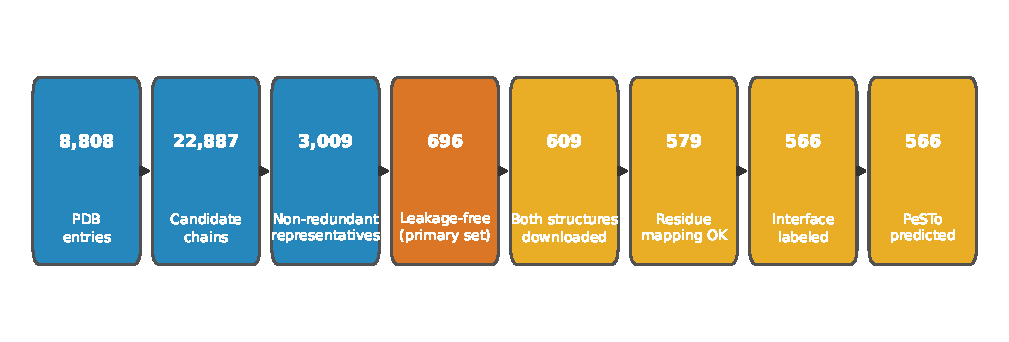
\includegraphics[width=\textwidth]{figures/fig1_attrition.pdf}
\caption{Dataset construction: candidate PDB chains are reduced by
redundancy clustering, sequence-level leakage filtering against PeSTo's own
training/validation/test data, structure availability, residue-mapping
validation, and interface labeling, to the 566-chain primary
benchmark set. Counts are for the primary (leakage-filtered) track only.}
\label{fig:attrition}
\end{figure}

\subsection{Inference}

The pretrained PeSTo model (its element-only-input variant) was run on each of
the 566 primary-set chains in two input forms: the isolated
experimental chain (\emph{exp}), and the AlphaFold model trimmed to the same
mapped residue range (\emph{af\_trimmed}). Both runs used the chain in
isolation, with no partner structure present, matching how an interface
predictor would be applied to a single AlphaFold model in practice.

\subsection{Pre-registered analysis plans}

Two analyses were pre-registered in writing, with endpoints and thresholds
fixed before either was run against real predictions.

\textbf{Benchmark (Section~3.1).} Primary and secondary endpoints are the
paired per-chain difference (experimental minus AlphaFold-trimmed) in AUPR and
ROC-AUC respectively, restricted to chains where both metrics are defined
(excluding chains whose scored residues are single-class); tested with a
two-sided Wilcoxon signed-rank test and a chain-resampled 95\% bootstrap CI on
the median difference (10,000 resamples, chains, not residues,
resampled with replacement, since residues within one chain are not
independent observations). Four descriptive strata (homomeric vs.\
heteromeric partner, small vs.\ large interface fraction, chains geometrically
flagged by an independent AlphaFold-vs-experimental superposition check vs.\
not, all residues vs.\ surface residues only) and a robustness check against
the buried-surface-area label were specified alongside the primary endpoint,
not as additional hypothesis tests.

\textbf{Error analysis (Section~3.2).} pLDDT confidence bands are fixed at
50, 70, 90 (AlphaFold's own convention), with pooled AUPR/ROC-AUC
computed for both inputs within each band and a chain-resampled bootstrap CI
(2,000 resamples per band, fewer than the benchmark's
10,000 because each draw here recomputes a full pooled metric over
tens of thousands of residues rather than a cheap scalar). A per-residue
regression relates the absolute prediction shift, $|p_{\mathrm{AF}} -
p_{\mathrm{exp}}|$, to standardized pLDDT, standardized local C$\alpha$ RMSD,
standardized relative solvent accessibility (RSA), and secondary-structure
class (coil as reference), with cluster-robust standard errors clustered by
chain and variance inflation factors (VIF) reported for each predictor
(flagged above 5, since pLDDT and local RMSD are both proxies
for the same underlying AlphaFold-vs-experimental divergence and are expected
to correlate). Local RMSD is computed with a separate rigid-body superposition
per residue's own 10\,\r{A} neighborhood, rather than one
superposition for the whole chain, so that structural motion elsewhere in a
multi-domain chain is not mistaken for local error at a given residue.
Descriptive analyses of chain length and of the geometrically flagged chains
were specified as associations to be reported, not confirmatory tests.

\section{Results}

\subsection{Benchmark: experimental versus AlphaFold-trimmed input}

Of the 566 primary-set chains, 12 (2.1\%)
were excluded from every paired comparison because every scored residue in
the chain was labeled interface, leaving no non-interface residues against
which to compute ROC-AUC or AUPR; the remaining 554 chains form the
primary comparison.

PeSTo was more accurate on experimental input than on the matched
AlphaFold-trimmed input: the median paired AUPR difference was
0.027 (95\% CI [0.019, 0.035], Wilcoxon $p=$$3.5\times10^{-17}$), and
the paired ROC-AUC difference showed the same pattern (median
0.027, CI [0.018, 0.037], $p=$$4.6\times10^{-19}$). Pooling all
95,118 scored residues (interface base rate 0.223)
rather than comparing per-chain gives AUPR 0.739 on
experimental input versus 0.669 on AlphaFold input (pooled
ROC-AUC 0.882 vs.\ 0.849) -- both inputs are far
above the base rate, so both are informative, but the pooled AUPR gap
(0.070) is noticeably larger than the per-chain median gap;
Section~3.2 returns to why. Replacing the distance-based interface label with
the buried-surface-area label reproduces essentially the same result (median
0.026, CI [0.020, 0.034], $p=$$3.0\times10^{-17}$), so the finding is not
an artifact of the distance-cutoff label definition.

\begin{figure}[t]
\centering
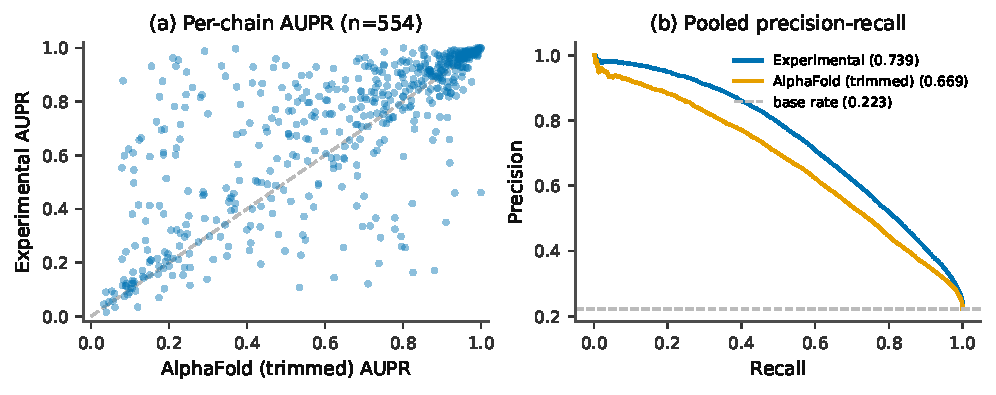
\includegraphics[width=\textwidth]{figures/fig2_phase7_primary.pdf}
\caption{(a) Per-chain AUPR, experimental vs.\ AlphaFold-trimmed input; most
chains sit near the identity line with a tilt toward experimental input, and a
right-skewed tail where AlphaFold input costs noticeably more accuracy. (b)
Precision--recall curves pooling every scored residue in the primary set,
for each input, against the pooled interface base rate.}
\label{fig:phase7primary}
\end{figure}

All eight pre-registered strata showed the same direction of effect (Fig.~\ref{fig:strata}),
from a median 0.015 ($n=$120, Interface fraction $\geq$ 0.5)
to 0.059 ($n=$92, Geometrically flagged); none
reversed sign or lost significance in either direction. The gap is therefore
not confined to one kind of chain, though its size varies noticeably --
largest among the minority of chains flagged by an independent geometric
check as showing unusual 3D disagreement between the AlphaFold model and the
experimental structure.

\begin{figure}[t]
\centering
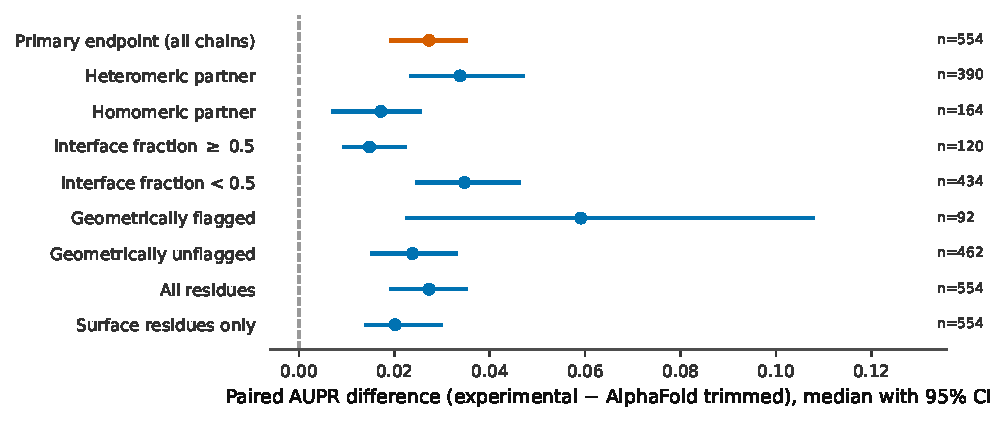
\includegraphics[width=\textwidth]{figures/fig3_phase7_strata.pdf}
\caption{Paired AUPR difference (median, 95\% chain-resampled bootstrap CI)
for the primary endpoint and each of the eight pre-registered descriptive
strata. All intervals lie on the same side of zero.}
\label{fig:strata}
\end{figure}

\subsection{Error analysis: what the gap is associated with}

Stratifying every scored residue by AlphaFold's own pLDDT confidence band
(Fig.~\ref{fig:bands}, Table~\ref{tab:bands}) shows the AUPR gap shrinking
monotonically as confidence increases, from 0.254 in the lowest band to
0.039 in the highest -- roughly a 6.4-fold reduction -- with
the same pattern in ROC-AUC. Every band cleared the minimum-residue reporting
threshold with no undefined bootstrap draws.

\begin{figure}[t]
\centering
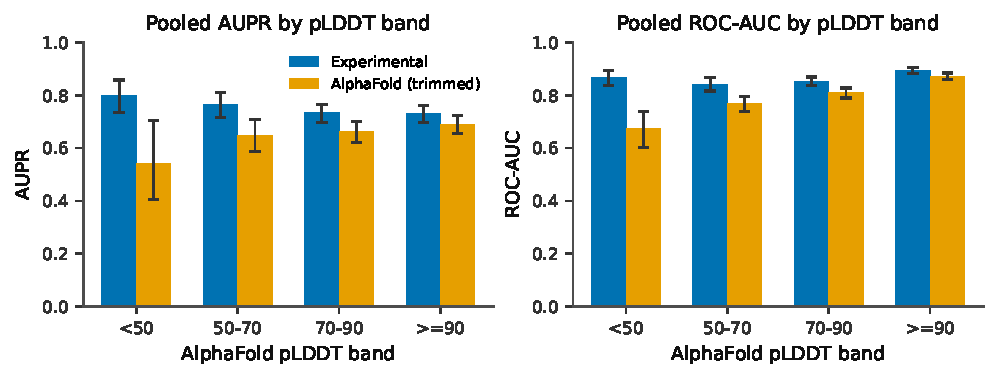
\includegraphics[width=\textwidth]{figures/fig4_phase8_bands.pdf}
\caption{Pooled AUPR and ROC-AUC by AlphaFold pLDDT confidence band, both
inputs, with 95\% chain-resampled bootstrap CIs. The experimental-vs.-AlphaFold
gap is largest in AlphaFold's least confident residues and smallest in its
most confident ones.}
\label{fig:bands}
\end{figure}

\begin{table}[t]
\centering
\small
\begin{tabular}{lrrlrlrl}
\toprule
Band & $n$ res. & $n$ ch. & Base rate & Input & ROC-AUC (95\% CI) & \multicolumn{2}{l}{AUPR (95\% CI)} \\
\midrule
<50 & 2,828 & 216 & 0.400 & Experimental & 0.868 [0.836, 0.894] & \multicolumn{2}{l}{0.798 [0.734, 0.858]} \\
 &  &  &  & AlphaFold trimmed & 0.673 [0.602, 0.738] & \multicolumn{2}{l}{0.543 [0.406, 0.705]} \\
\addlinespace
50-70 & 5,735 & 445 & 0.332 & Experimental & 0.843 [0.816, 0.867] & \multicolumn{2}{l}{0.766 [0.717, 0.810]} \\
 &  &  &  & AlphaFold trimmed & 0.768 [0.737, 0.797] & \multicolumn{2}{l}{0.649 [0.587, 0.707]} \\
\addlinespace
70-90 & 23,762 & 535 & 0.256 & Experimental & 0.853 [0.836, 0.869] & \multicolumn{2}{l}{0.734 [0.699, 0.766]} \\
 &  &  &  & AlphaFold trimmed & 0.809 [0.790, 0.828] & \multicolumn{2}{l}{0.663 [0.623, 0.701]} \\
\addlinespace
>=90 & 62,793 & 493 & 0.192 & Experimental & 0.893 [0.882, 0.904] & \multicolumn{2}{l}{0.730 [0.697, 0.761]} \\
 &  &  &  & AlphaFold trimmed & 0.871 [0.858, 0.885] & \multicolumn{2}{l}{0.690 [0.655, 0.724]} \\
\bottomrule
\end{tabular}
\caption{Pooled ROC-AUC and AUPR by pLDDT band, both inputs, with 95\%
chain-resampled bootstrap CIs.}
\label{tab:bands}
\end{table}

A per-residue regression of the absolute prediction shift on standardized
pLDDT, local RMSD, RSA, and secondary structure (Fig.~\ref{fig:regression},
Table~\ref{tab:regression}; $n=$95,117 of the 95,118 pooled
residues -- 1 excluded for a missing RSA value, a single
non-standard N-terminal residue whose chemical component has no Sander/Rost
reference accessible-surface-area value, logged during Phase 5 and not
otherwise informative for this regression -- 566 chain
clusters, cluster-robust standard errors) finds pLDDT
(coefficient -0.0268, $p=$$3.9\times10^{-16}$) and local RMSD (coefficient
0.0268, $p=$$1.4\times10^{-9}$) each independently associated with the size of
the shift in the expected direction -- higher confidence is associated with a
smaller shift, larger local structural divergence with a larger one -- after
controlling for the other and for RSA (coefficient 0.0254,
$p=$$1.4\times10^{-57}$). No predictor's variance inflation factor exceeded
5 (maximum 1.64): despite both being proxies for
AlphaFold-vs-experimental divergence, pLDDT and local RMSD carry only mild
collinearity here and each retains independent explanatory power. Consistent
with the shift regression, mean absolute prediction shift rises steadily with
local RMSD (Fig.~\ref{fig:regression}a).

\begin{figure}[t]
\centering
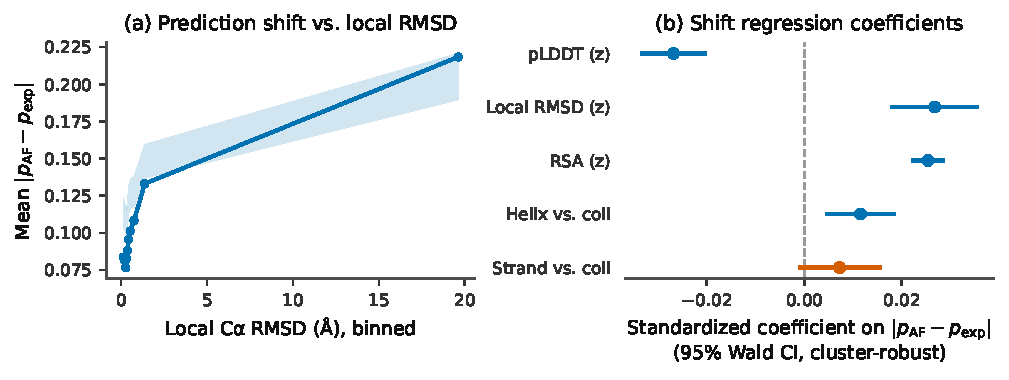
\includegraphics[width=\textwidth]{figures/fig5_phase8_regression.pdf}
\caption{(a) Mean absolute prediction shift by binned local C$\alpha$ RMSD,
with chain-resampled 95\% CIs. (b) Standardized coefficients (95\% Wald CI)
from the per-residue shift regression; grey markers did not reach $p<0.05$.}
\label{fig:regression}
\end{figure}

\begin{table}[t]
\centering
\small
\begin{tabular}{lrrrrr}
\toprule
Term & Coef. & Cluster-robust SE & $t$ & $p$ & VIF \\
\midrule
Intercept & 0.1019 & 0.0029 & 35.17 & $6.8\times10^{-271}$ & -- \\
pLDDT (z) & -0.0268 & 0.0033 & -8.14 & $3.9\times10^{-16}$ & 1.64 \\
Local RMSD (z) & 0.0268 & 0.0044 & 6.05 & $1.4\times10^{-9}$ & 1.48 \\
RSA (z) & 0.0254 & 0.0016 & 15.99 & $1.4\times10^{-57}$ & 1.18 \\
Helix vs. coil & 0.0115 & 0.0035 & 3.30 & $9.8\times10^{-4}$ & 1.15 \\
Strand vs. coil & 0.0073 & 0.0042 & 1.74 & $0.081$ & 1.18 \\
\bottomrule
\end{tabular}
\caption{Regression of $|p_{\mathrm{AF}}-p_{\mathrm{exp}}|$ on standardized
predictors, cluster-robust standard errors by chain.
Reference category: secondary structure = coil.}
\label{tab:regression}
\end{table}

Two pre-registered descriptive analyses addressed possible confounds. First,
per-chain AUPR drop showed no meaningful association with chain length
(Spearman $\rho=$0.028, 95\% CI [-0.054, 0.108], $p=$0.51) -- this
contradicts the pre-registration's stated expectation that chain length would
explain why the pooled AUPR gap (0.070) exceeds the per-chain
median gap (0.027); the actual explanation is that the drop
distribution is right-skewed (unweighted mean 0.061 vs.\
median 0.027), and weighting the mean by chain length
barely moves it (0.061) -- a minority of chains with an
unusually large drop pull the mean well above the median, not long chains in
general. Second, the 92 chains geometrically flagged for unusual
3D disagreement between AlphaFold and the experimental structure differ from
the remaining 462 on every structural measure examined
(Table~\ref{tab:flagged}): substantially lower mean pLDDT ($p=$$2.8\times10^{-11}$)
and higher local RMSD ($p=$$4.2\times10^{-32}$), consistent with this flag
capturing genuine AlphaFold-vs-experimental divergence rather than a mapping
artifact.

\begin{table}[t]
\centering
\small
\begin{tabular}{lrrr}
\toprule
Metric & Flagged mean (median) & Unflagged mean (median) & $p$ \\
\midrule
Per-chain AUPR drop & 0.108 (0.0591) & 0.052 (0.0238) & $0.020$ \\
Chain length (residues) & 224 (202) & 162 (117) & $2.5\times10^{-4}$ \\
Interface fraction & 0.314 (0.215) & 0.327 (0.266) & $0.179$ \\
Mean pLDDT & 77.4 (84.1) & 87.9 (90.6) & $2.8\times10^{-11}$ \\
Mean local RMSD (\r{A}) & 2.21 (1.39) & 0.672 (0.55) & $4.2\times10^{-32}$ \\
Mean global C$\alpha$ dist. (\r{A}) & 7.91 (7.37) & 1.4 (0.98) & $9.5\times10^{-40}$ \\
\bottomrule
\end{tabular}
\caption{Geometrically flagged vs.\ unflagged primary-set chains
(two-sided Mann-Whitney $U$ test).}
\label{tab:flagged}
\end{table}

Figure~\ref{fig:structure} illustrates these results on a single chain
(PDB 7DZ9, chain C, UniProt E3BK13,
180 residues), chosen because its AUPR drop (0.031) sits close to
the primary endpoint's median. PeSTo's experimental-input predictions
(AUPR 0.837) track the true interface patch more tightly than its
AlphaFold-input predictions (AUPR 0.806) on the same residues, though
both visibly recover the same overall interface region.

\begin{figure}[t]
\centering
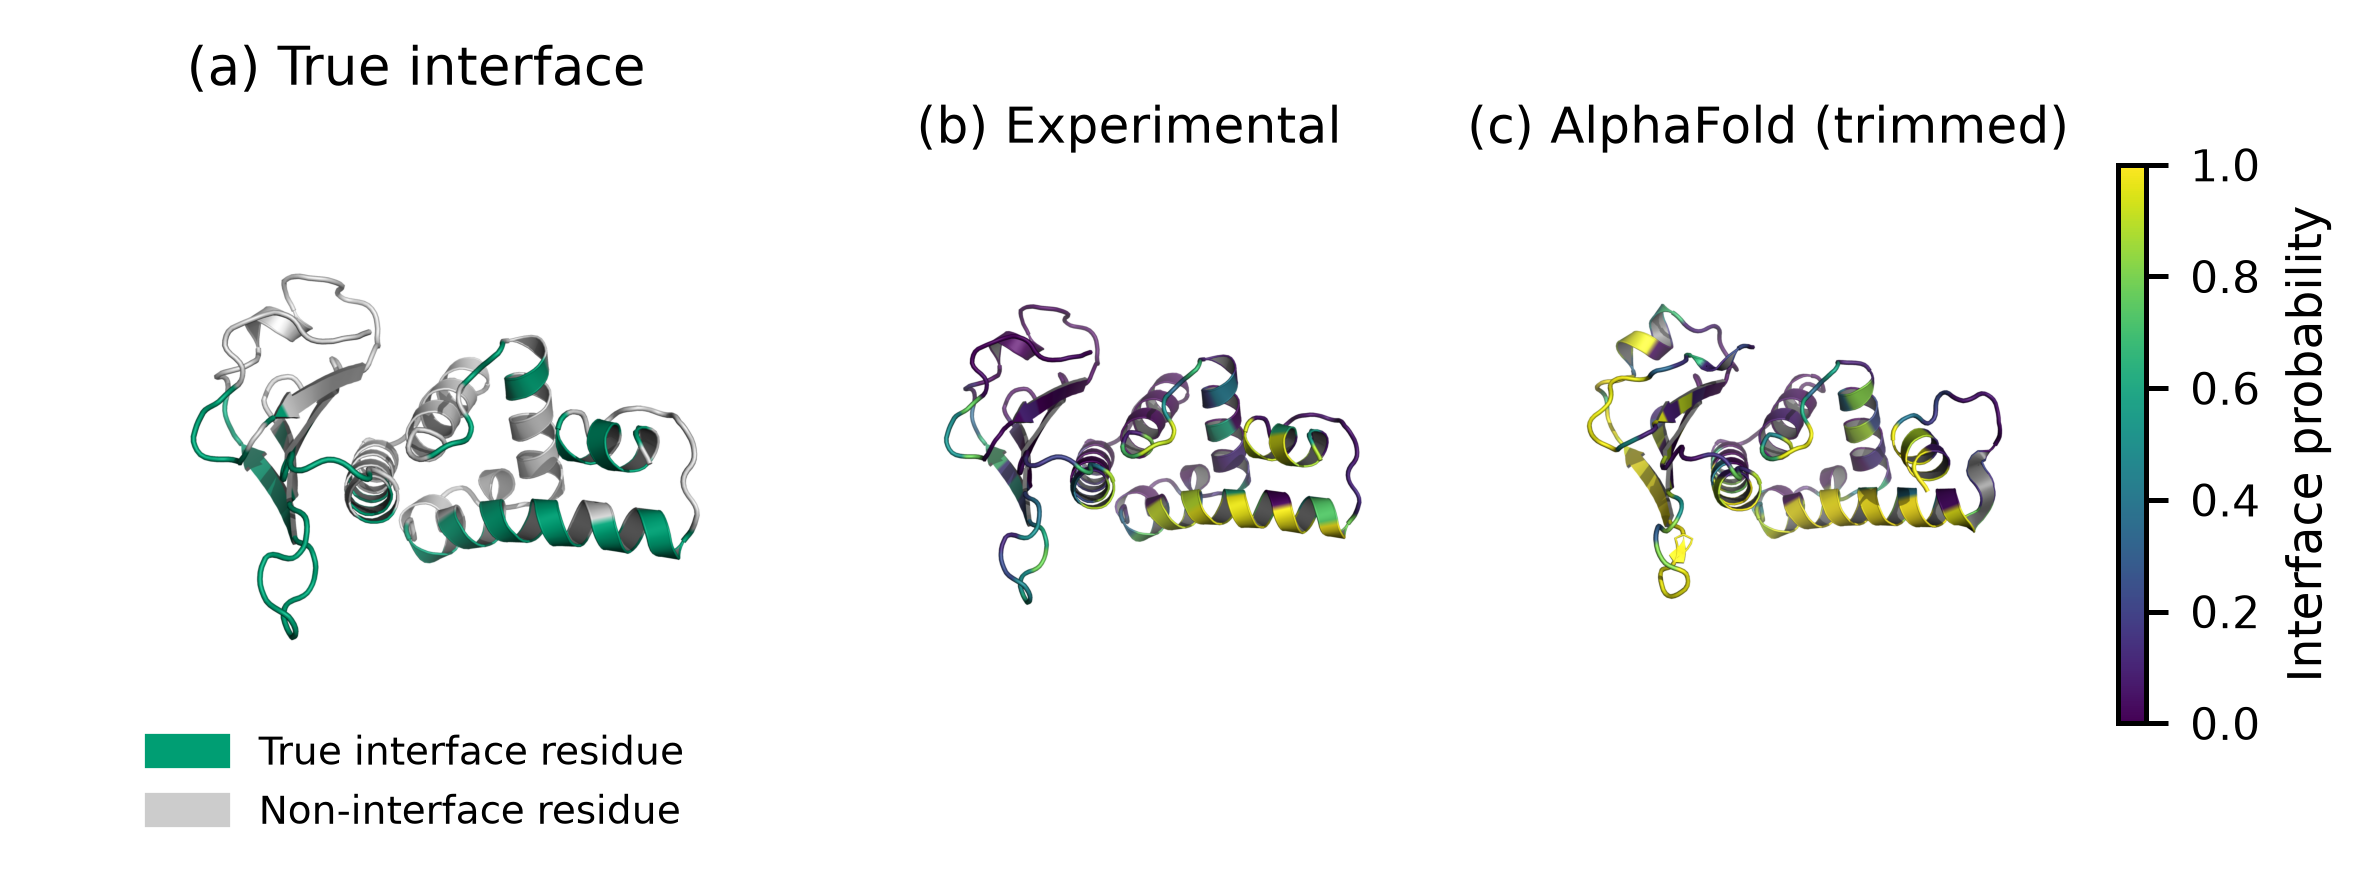
\includegraphics[width=0.92\textwidth]{figures/example_chain_render.png}
\caption{A representative chain (rendered with PyMOL (cartoon representation), not a C$\alpha$ trace; the AlphaFold model in (c) is Kabsch-superposed onto the experimental structure and all three panels share one camera orientation -- see scripts/render\_example\_chain.py and the accompanying repository's README.md for how this image was produced).
(a) True interface residues (green) vs.\ non-interface (grey). (b) PeSTo's
per-residue interface probability from the experimental structure
(AUPR 0.837 on this chain). (c) PeSTo's per-residue interface
probability from the AlphaFold model trimmed to the same residues
(AUPR 0.806), superposed onto the experimental frame for comparison
only (the underlying coordinates, and hence the prediction, come from the
AlphaFold model).}
\label{fig:structure}
\end{figure}

\subsection{Does pLDDT filtering actually help? (post-hoc, exploratory)}

Section~3.2's regression shows pLDDT is \emph{associated} with the size of
the prediction shift, but that does not by itself establish that discarding
low-pLDDT residues is a good deployment rule. This subsection tests that
directly. It was not pre-registered before Phase 7/8 were run -- the
motivating question only arose from their results -- so it is reported here
as a post-hoc, exploratory check (pre-registered in writing before these
specific numbers were computed; see PLAN.md's Phase 8b), not as confirmatory
evidence.

For both inputs, at a fixed probability threshold (0.5,
not tuned per input or cutoff) we swept a pLDDT cutoff
(0, 50, 70, 90) that discards
residues below it, and recomputed precision, recall, and F1 on what
remains (Table~\ref{tab:filtering}, Fig.~\ref{fig:filtering}). The
identical sweep on \emph{experimental} input serves as a reference. Since
pLDDT is a property of the AlphaFold model shared by both inputs' rows, any
F1 change on the \emph{exp} curve reflects only the generic effect of
discarding residues, not anything specific to AlphaFold's structural
error -- comparing the two curves isolates the latter.

Filtering at 90 discards 34\%
of all residues and, importantly, 43\% of the
true interface residues, while moving AlphaFold-input F1 from
0.596 (CI [0.571, 0.621]) to only
0.603 (CI [0.573, 0.633]) -- an absolute gain of
0.007, with overlapping confidence intervals, i.e. not
clearly distinguishable from no improvement at all. The gap to experimental
input's F1 narrows only slightly, from 0.050 at no filtering to
0.031 at the strictest cutoff, and part of even that narrowing
is experimental input's own F1 drifting down (0.647 to
0.634) as its harder, lower-pLDDT residues are discarded too
-- not AlphaFold input distinctly "catching up." The composition of the
small gain is also informative: AlphaFold-input precision rises from
0.673 to 0.713 while recall is
essentially flat (0.535 to 0.523) --
filtering trades a large, real cost in discarded true interface residues
for a modest precision gain, not a broad quality improvement. At a fixed
0.5 threshold, pLDDT filtering does not meaningfully close the
experimental-vs-AlphaFold gap, and its practical benefit here is limited
relative to its cost.

\begin{figure}[t]
\centering
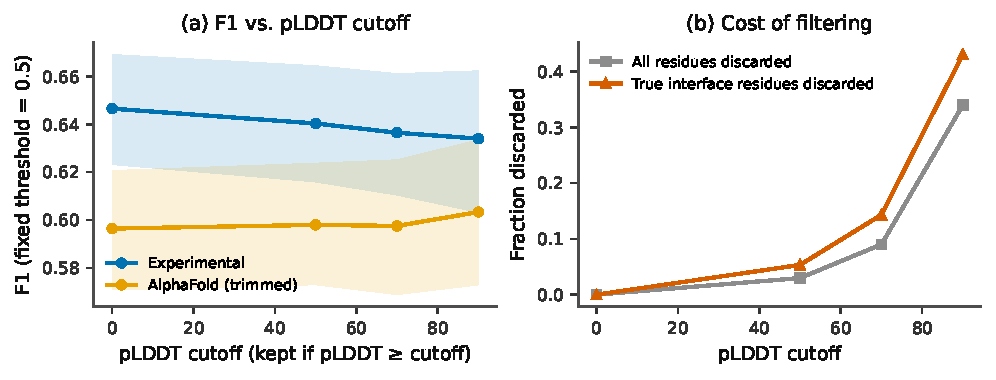
\includegraphics[width=\textwidth]{figures/fig7_plddt_filtering.pdf}
\caption{(a) F1 at a fixed 0.5 probability threshold vs.\ pLDDT cutoff, both
inputs, with 95\% chain-resampled bootstrap CIs. (b) Fraction of all
residues, and of true interface residues specifically, discarded at each
cutoff (identical for both inputs, since pLDDT is a property of the
AlphaFold model, not of which input is scored).}
\label{fig:filtering}
\end{figure}

\begin{table}[t]
\centering
\footnotesize
\begin{tabular}{lrrrlll}
\toprule
Input & Cutoff & \% res. kept & \% interface kept & Precision (95\% CI) & Recall (95\% CI) & F1 (95\% CI) \\
\midrule
Experimental & 0 & 100.0 & 100.0 & 0.73 [0.71, 0.75] & 0.58 [0.55, 0.61] & 0.65 [0.62, 0.67] \\
AlphaFold trimmed &  & 100.0 & 100.0 & 0.67 [0.65, 0.70] & 0.54 [0.50, 0.57] & 0.60 [0.57, 0.62] \\
\addlinespace
Experimental & 50 & 97.0 & 94.7 & 0.73 [0.70, 0.75] & 0.57 [0.54, 0.60] & 0.64 [0.62, 0.66] \\
AlphaFold trimmed &  & 97.0 & 94.7 & 0.69 [0.66, 0.71] & 0.53 [0.50, 0.56] & 0.60 [0.57, 0.62] \\
\addlinespace
Experimental & 70 & 91.0 & 85.7 & 0.73 [0.70, 0.75] & 0.57 [0.54, 0.60] & 0.64 [0.61, 0.66] \\
AlphaFold trimmed &  & 91.0 & 85.7 & 0.69 [0.67, 0.72] & 0.52 [0.49, 0.56] & 0.60 [0.57, 0.63] \\
\addlinespace
Experimental & 90 & 66.0 & 57.0 & 0.74 [0.71, 0.77] & 0.56 [0.52, 0.59] & 0.63 [0.60, 0.66] \\
AlphaFold trimmed &  & 66.0 & 57.0 & 0.71 [0.68, 0.74] & 0.52 [0.49, 0.56] & 0.60 [0.57, 0.63] \\
\bottomrule
\end{tabular}
\caption{Precision/recall/F1 (fixed 0.5 threshold) by pLDDT cutoff, both
inputs, with 95\% chain-resampled bootstrap CIs. Post-hoc, exploratory
(Section~3.3).}
\label{tab:filtering}
\end{table}

\section{Discussion}

In practical terms, PeSTo's accuracy cost from using an AlphaFold structure
instead of an experimental one is real, directionally consistent, and
statistically unambiguous, but modest for a typical chain: a median AUPR
difference around 0.027 on a 0--1 scale is a small-to-moderate
effect, not a collapse in accuracy, and Fig.~\ref{fig:phase7primary}a shows
most chains clustering close to the identity line. The pooled-residue
comparison (0.739 vs.\ 0.669) paints a
superficially larger gap, but Section~3.2 shows that gap is driven by a
right-skewed minority of chains rather than a uniform shift, so reporting the
per-chain median alongside the pooled number matters for not overstating the
typical case.

This project's numbers are not directly comparable to Yuan et al.'s
ESMFold-based benchmark (0.797 to 0.691 AUPR) \cite{yuan2024}: the structure
predictor, the candidate set, the leakage control, and the interface
definition all differ, and only the direction of the effect -- a real
accuracy cost from using a predicted structure -- is expected to generalize
between the two studies, not the magnitude. AlphaFold's average accuracy is
generally reported as higher than ESMFold's \cite{lin2023}, which is at least
directionally consistent with this study's smaller median per-chain gap, but
the two benchmarks differ in enough other respects (dataset, leakage
definition, exact interface criterion) that this is a plausible reading of
the comparison, not a controlled one.

The error analysis in Section~3.2 points to a specific, mechanistic account
of the gap rather than a diffuse "AlphaFold structures are worse" story: the
accuracy cost concentrates in residues where AlphaFold itself reports low
confidence and where the local backbone geometry genuinely diverges from the
experimental structure, and these two signals carry largely independent
information (low collinearity despite both tracking the same underlying
divergence). But association with a continuous shift is not the same as a
useful deployment rule, and Section~3.3's direct test of the natural
follow-on idea -- discard low-pLDDT residues before trusting AlphaFold-input
predictions -- found limited practical benefit at a fixed threshold: F1
improved by only 0.007 from no filtering to the strictest
cutoff, well within overlapping confidence intervals of no improvement at
all, while discarding 43\% of the true
interface residues in the process. pLDDT is a real, independent correlate
of where predictions shift the most; that is a weaker and more qualified
claim than a validated confidence-based filter, and this paper does not
claim the latter.

\section{Limitations}

\begin{itemize}[nosep,leftmargin=1.4em]
\item \textbf{Temporal skew.} The primary set's leakage-filtering requirement
(sequence identity below 30\% against PeSTo's training
data) leaves it skewed toward chains released in 2021 or later, farther in
time from AlphaFold's 2018-04-30 cutoff than the filter alone requires; PeSTo's
own training-data snapshot appears to extend to roughly 2020--2021, later
than AlphaFold2's cutoff, based on a release-year breakdown of the leakage
flag (not shown here).
\item \textbf{Bound vs.\ unbound conformations.} Both experimental structures
here are \emph{bound}, complexed structures; a protein's shape can change
somewhat upon binding, and this study cannot separate that ordinary
conformational change from AlphaFold-specific structural error, because the
independently solved unbound (apo) arm designed to make that separation was
not run in this pass.
\item \textbf{Deferred comparisons.} The untrimmed, full-length AlphaFold
model (as opposed to the same model trimmed to the experimentally observed
range) and the leakage-sensitivity subsets at looser identity thresholds were
not run in this pass; the trimmed-model result reported here should not be
read as characterizing performance on a full-length AlphaFold model used
without any trimming.
\item \textbf{Single predictor, single confidence signal.} All results are
specific to PeSTo; whether they generalize to ScanNet \cite{tubiana2022},
HIGH-PPI \cite{gao2023}, or other interface predictors is untested here. Only pLDDT was used as AlphaFold's
confidence signal; predicted aligned error (PAE), which is specific to
multi-chain predictions, was not available since every AlphaFold input here
is a single trimmed monomer model.
\item \textbf{Monomeric AlphaFold models.} Every AlphaFold structure used here
is a single-chain model; no multi-chain (complex) AlphaFold prediction was
evaluated, so this study speaks to isolated-chain structure quality, not to
whether an AlphaFold-predicted complex's own interface would look different.
\end{itemize}

\section{Future Work}

The deferred arms noted above -- the untrimmed full-length AlphaFold
comparison, the unbound/apo arm, and the leakage-sensitivity subsets at looser
identity thresholds -- remain natural next steps and require no new method,
only additional runs of the existing pipeline. Section~3.3 found that simply
\emph{discarding} low-pLDDT residues at a fixed threshold recovers little of
the measured accuracy cost, which is itself informative: it suggests the
useful information in pLDDT is more continuous than a hard cutoff can
exploit. A pLDDT-\emph{aware} fine-tuning of PeSTo -- adding pLDDT as an
extra per-residue input channel, training on a mixed set of experimental
structures (pLDDT fixed at 100) and AlphaFold structures (their real pLDDT)
-- remains a plausible next step, since a trained model could in principle
learn a more graded use of the signal than any fixed cutoff; but Section~3.3
means this should be treated as an open question to test, not a predicted
win.

\bibliographystyle{plain}
\begin{thebibliography}{9}

\bibitem{zhang2024} Zhang, J., Durham, J., Cong, Q. Revolutionizing
protein--protein interaction prediction with deep learning. \emph{Curr Opin
Struct Biol} \textbf{85}, 102775 (2024).
\url{https://doi.org/10.1016/j.sbi.2024.102775}

\bibitem{jumper2021} Jumper, J.\ et al.\ Highly accurate protein structure
prediction with AlphaFold. \emph{Nature} \textbf{596}, 583--589 (2021).
\url{https://doi.org/10.1038/s41586-021-03819-2}

\bibitem{varadi2024} Varadi, M.\ et al.\ AlphaFold Protein Structure Database
in 2024: providing structure coverage for over 214 million protein sequences.
\emph{Nucleic Acids Res} \textbf{52}, D368--D375 (2024).
\url{https://doi.org/10.1093/nar/gkad1011}

\bibitem{krapp2023} Krapp, L.F., Abriata, L.A., Cort\'es Rodr\'iguez, F.\ et
al.\ PeSTo: parameter-free geometric deep learning for accurate prediction of
protein binding interfaces. \emph{Nat Commun} \textbf{14}, 2175 (2023).
\url{https://doi.org/10.1038/s41467-023-37701-8}

\bibitem{tubiana2022} Tubiana, J., Schneidman-Duhovny, D., Wolfson, H.J.
ScanNet: an interpretable geometric deep learning model for structure-based
protein binding site prediction. \emph{Nat Methods} \textbf{19}, 730--739
(2022). \url{https://doi.org/10.1038/s41592-022-01490-7}

\bibitem{terwilliger2024} Terwilliger, T.C.\ et al.\ AlphaFold predictions are
valuable hypotheses and accelerate but do not replace experimental structure
determination. \emph{Nat Methods} \textbf{21}, 110--116 (2024).
\url{https://doi.org/10.1038/s41592-023-02087-4}

\bibitem{yuan2024} Yuan, Q.\ et al.\ Genome-scale annotation of protein
binding sites via language model and geometric deep learning. \emph{eLife}
\textbf{13}, e93695 (2024). \url{https://doi.org/10.7554/eLife.93695}

\bibitem{lin2023} Lin, Z.\ et al.\ Evolutionary-scale prediction of
atomic-level protein structure with a language model. \emph{Science}
\textbf{379}, 1123--1130 (2023). \url{https://doi.org/10.1126/science.ade2574}

\bibitem{krissinel2007} Krissinel, E., Henrick, K. Inference of macromolecular
assemblies from crystalline state. \emph{J Mol Biol} \textbf{372}, 774--797
(2007). \url{https://doi.org/10.1016/j.jmb.2007.05.022}

\bibitem{gao2023} Gao, Z., Jiang, C., Zhang, J.\ et al.\ Hierarchical graph
learning for protein--protein interaction. \emph{Nat Commun} \textbf{14}, 1093
(2023). \url{https://doi.org/10.1038/s41467-023-36736-1}

\end{thebibliography}

\end{document}
